\documentclass[10pt]{beamer}
\usetheme[
%%% options passed to the outer theme
%    hidetitle,           % hide the (short) title in the sidebar
%    hideauthor,          % hide the (short) author in the sidebar
%    hideinstitute,       % hide the (short) institute in the bottom of the sidebar
%    shownavsym,          % show the navigation symbols
%    width=2cm,           % width of the sidebar (default is 2 cm)
    hideothersubsections,% hide all subsections but the subsections in the current section
%    hideallsubsections,  % hide all subsections
    left               % right of left position of sidebar (default is right)
%%% options passed to the color theme
%    lightheaderbg,       % use a light header background
  ]{AAUsidebar}

% If you want to change the colors of the various elements in the theme, edit and uncomment the following lines
% Change the bar and sidebar colors:
%\setbeamercolor{AAUsidebar}{fg=red!20,bg=red}
%\setbeamercolor{sidebar}{bg=red!20}
% Change the color of the structural elements:
%\setbeamercolor{structure}{fg=red}
% Change the frame title text color:
%\setbeamercolor{frametitle}{fg=blue}
% Change the normal text color background:
%\setbeamercolor{normal text}{bg=gray!10}
% ... and you can of course change a lot more - see the beamer user manual.


\usepackage[utf8]{inputenc}
\usepackage[english]{babel}
\usepackage[T1]{fontenc}
% Or whatever. Note that the encoding and the font should match. If T1
% does not look nice, try deleting the line with the fontenc.
\usepackage{helvet}
\usepackage{listings}
\usepackage{color}
\definecolor{mygreen}{rgb}{0,0.6,0}
\definecolor{mygray}{rgb}{0.5,0.5,0.5}
\definecolor{bluekeywords}{rgb}{0.13,0.13,1}
\definecolor{redstring}{rgb}{0.6,0,0}
\definecolor{javaKeywords}{HTML}{7F0055}
\definecolor{diff}{HTML}{c5c5c5}

\lstdefinestyle{nc}%
{
  %morecomment  = [l]{//},
  morecomment  = [l][\nullfont]{//},
  morecomment  = [is]{/*}{*/}
}

\lstset{ %
  backgroundcolor=\color{white},   % choose the background color; you must add \usepackage{color} or \usepackage{xcolor}
  basicstyle=\scriptsize,        % the size of the fonts that are used for the
  % code
  breakatwhitespace=false,         % sets if automatic breaks should only happen
  % % % at whitespace
  breaklines=true,                 % sets automatic line breaking
  captionpos=b,                    % sets the caption-position to bottom
  commentstyle=\color{mygreen},    % comment style
  deletekeywords={...},            % if you want to delete keywords from the given language
  keepspaces=true,                 % keeps spaces in text, useful for keeping
  columns=flexible,				  % indentation of code (possibly needs columns=flexible)
  language={Java},                 % the language of the code
  numbers=left,                    % where to put the line-numbers; possible values are (none, left, right)
  %numbersep=5pt,                   % how far the line-numbers are from the
  % code
  numberstyle=\tiny\color{black}, % the style that is used for the line-numbers
  showspaces=false,                % show spaces everywhere adding particular underscores; it overrides 'showstringspaces'
  showstringspaces=false,          % underline spaces within strings only
  showtabs=false,                  % show tabs within strings adding particular
  % underscores
  stepnumber=1,                    % the step between two line-numbers. If it's
  % 1, each line will be numbered
  keywordstyle=\color{javaKeywords}\bfseries,
  stringstyle=\color{bluekeywords},     % string literal style
  tabsize=4,                       % sets default tabsize to 2 spaces
  frame=single,
  style=nc,
  framesep=1pt,
  framexleftmargin=3pt,
  literate= {Å}{{\AA}}1 {å}{{\aa}}1 
}

% colored hyperlinks
\newcommand{\chref}[2]{%
  \href{#1}{{\usebeamercolor[bg]{AAUsidebar}#2}}%
}

\setcounter{tocdepth}{1}

\title[ARES]% optional, use only with long paper titles
{ARES}

  % could also be a conference name

\date{\today}

\author[] % optional, use only with lots of authors
{
Simon Højberg\\
Jonas Ibrahim\\
Jonathan Magnussen\\
Christoffer Mouritzen\\
Michael Sebastian Søby\\
Emil Hedeholm Sørensen\\
\href{mailto:sw507e16@cs.aau.dk}{{\tt sw507e16@cs.aau.dk}}
}
% - Give the names in the same order as they appear in the paper.
% - Use the \inst{?} command only if the authors have different
%   affiliation. See the beamer manual for an example

\institute[
%  {\includegraphics[scale=0.2]{aau_segl}}\\ %insert a company, department or university logo
  Dept.\ of Computer Science\\
  Aalborg University\\
  Denmark
] % optional - is placed in the bottom of the sidebar on every slide
{% is placed on the title page
  Department of Computer Science\\
  Aalborg University\\
  Denmark
  
  %there must be an empty line above this line - otherwise some unwanted space is added between the university and the country (I do not know why;( )
}


% specify a logo on the titlepage (you can specify additional logos an include them in 
% institute command below
\pgfdeclareimage[height=1.5cm]{titlepagelogo}{AAUgraphics/aau_logo_new} % placed on the title page
%\pgfdeclareimage[height=1.5cm]{titlepagelogo2}{graphics/aau_logo_new} % placed on the title page
\titlegraphic{% is placed on the bottom of the title page
  \pgfuseimage{titlepagelogo}
%  \hspace{1cm}\pgfuseimage{titlepagelogo2}
}


\begin{document}
% the titlepage
{\aauwavesbg%
\begin{frame}[plain,noframenumbering] % the plain option removes the sidebar and header from the title page
  \titlepage
\end{frame}}
%%%%%%%%%%%%%%%%

% TOC
\begin{frame}{Agenda}{}
\tableofcontents
\end{frame}

\section{Emil}
\begin{frame}{Emil}
\begin{itemize}
  \item Initial Problem and Ideal Scenario
  \item Intelligent Agents
  \item Hardware Choice
\end{itemize}
\end{frame}

\subsection{Initial Problem and Ideal Scenario}
\begin{frame}{Intial problem}
\begin{itemize}
\item How can an autonomous turret be designed and constructed such
that it is capable of hitting a moving target.
\end{itemize}
\end{frame}

\begin{frame}{Ideal scenario}
\begin{itemize}
  \item Scanning
  \item Tracking
  \item Shooting
\end{itemize}
\end{frame}

\begin{frame}{Embedded Systems}
\begin{itemize}
  \item Single functioned
  \item constrained
  \item reactive
\end{itemize}
\end{frame}

\subsection{Intelligent Agents}
\begin{frame}{Knowledge Representation}
\begin{itemize}
  \item Modelling the problem
  \item Choosing the right kind of solution
\end{itemize}
\end{frame}

\begin{frame}{Design space}
\begin{itemize}
\item Representation Scheme
\item Uncertainty
\end{itemize}
\end{frame}

\begin{frame}{Belief Network}
\begin{itemize}
 \item Why choose a Belief Network
 \item Hidden Markov Model
\end{itemize}
\end{frame}

\subsection{Hardware choice}
\begin{frame}{Platform Choice}
\begin{itemize}
 \item Criteria
 \item LEGO Mindstorms NXT
 \item Arduino
\end{itemize}
\end{frame}

\begin{frame}{sensor Choice}
\begin{itemize}
 \item Ultrasonic sensor
 \item Camera
\end{itemize}
\end{frame}
 

\section{Jonas}
%-------------------------------- FRAME 1 --------------------------------
\subsection{Overview}
\begin{frame}{Jonas: Overview}
\begin{itemize}
  \item Problem Statement
  		\begin{enumerate}
  			\item Features and Requirements
		\end{enumerate}
  \item Turret Design
  		\begin{enumerate}
  			\item Design Requirements
  			\item Turret Elements
  			\item Design Approaches
		\end{enumerate}
  \item Target Design
  		\begin{enumerate}
  			\item Movement
  		 	\item Trackability
		\end{enumerate}
\end{itemize}
\end{frame}

%-------------------------------- FRAME 2 --------------------------------
\subsection{Problem Statement}
\begin{frame}{Problem Statement}
\begin{center}
\begin{minipage}{0.8\linewidth}
\textit{How can an autonomous turret be constructed, designed and implemented
using the NXT, a camera and a pair of ultrasonic distance sensors. Furthermore,
how can a belief network be constructed and used for predicting the position
of the target.}
\end{minipage}
\end{center}
\end{frame}

\begin{frame}{Key Requirements}
\begin{itemize}
	\item Predict the targets future position
		\begin{itemize}
			\item Gather Data
			\item Calculate Position
		\end{itemize}
	\item Hit a moving target
		\begin{itemize}
			\item Move Into Position
			\item Fire at correct time
		\end{itemize}
	\item Make use of an MI model
\end{itemize}
\end{frame}

%-------------------------------- FRAME 3 --------------------------------
\subsection{Turret Design}
\begin{frame}{Turret Design}
\begin{itemize}
    \item Design Approaches
		\begin{enumerate}
  			\item Prototyping
  			\item Physical Limitations
  			\item Individual Part Design
		\end{enumerate} 
	\item Turret Parts
		\begin{enumerate}
  			\item Cannon
  			\item Frame
  			\item Rotation
		\end{enumerate}
\end{itemize}
\end{frame}

\begin{frame}{Cannon}

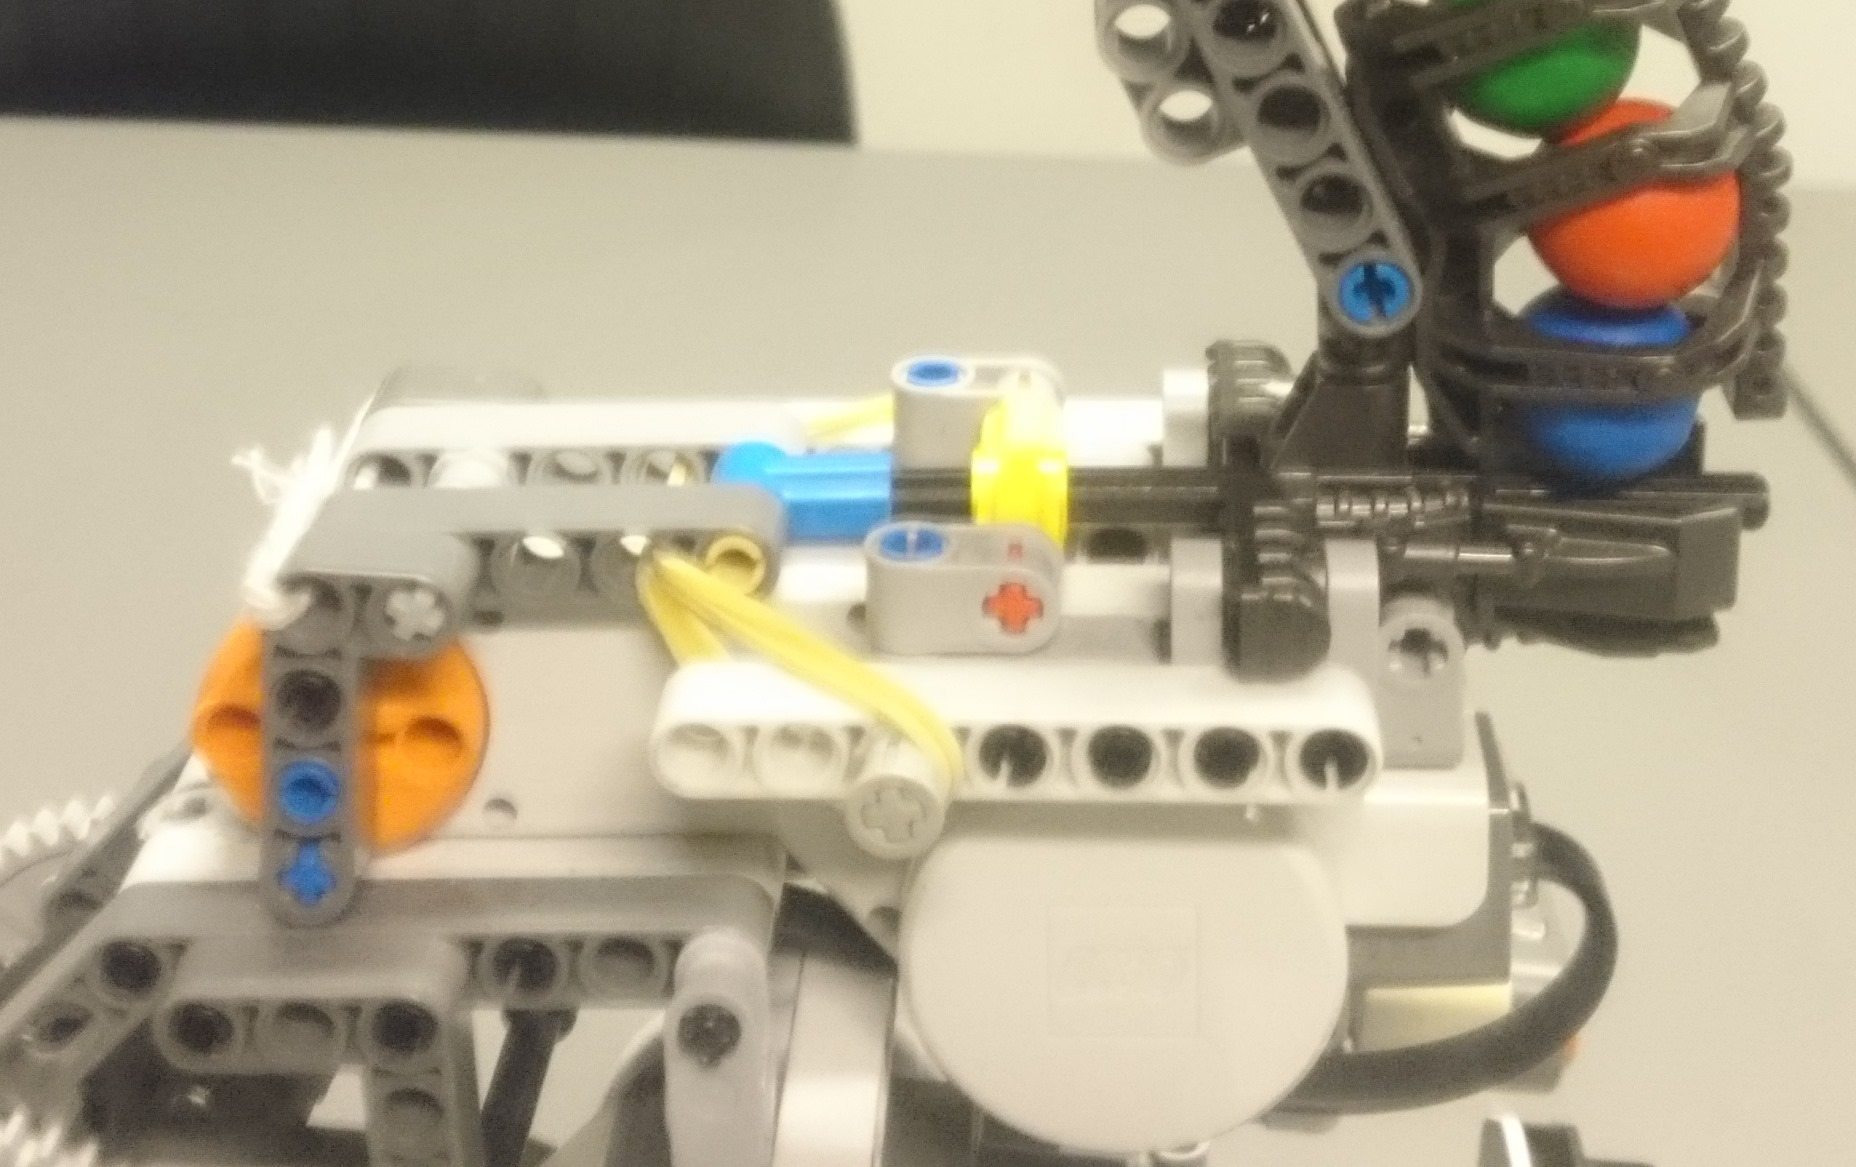
\includegraphics[scale=0.15]{figures/CannonMech.JPG} 

\begin{itemize}
	\item Ball Launcher
	\item Load / Reload
	\item Limited Power
\end{itemize}
\end{frame}

\begin{frame}{Frame}

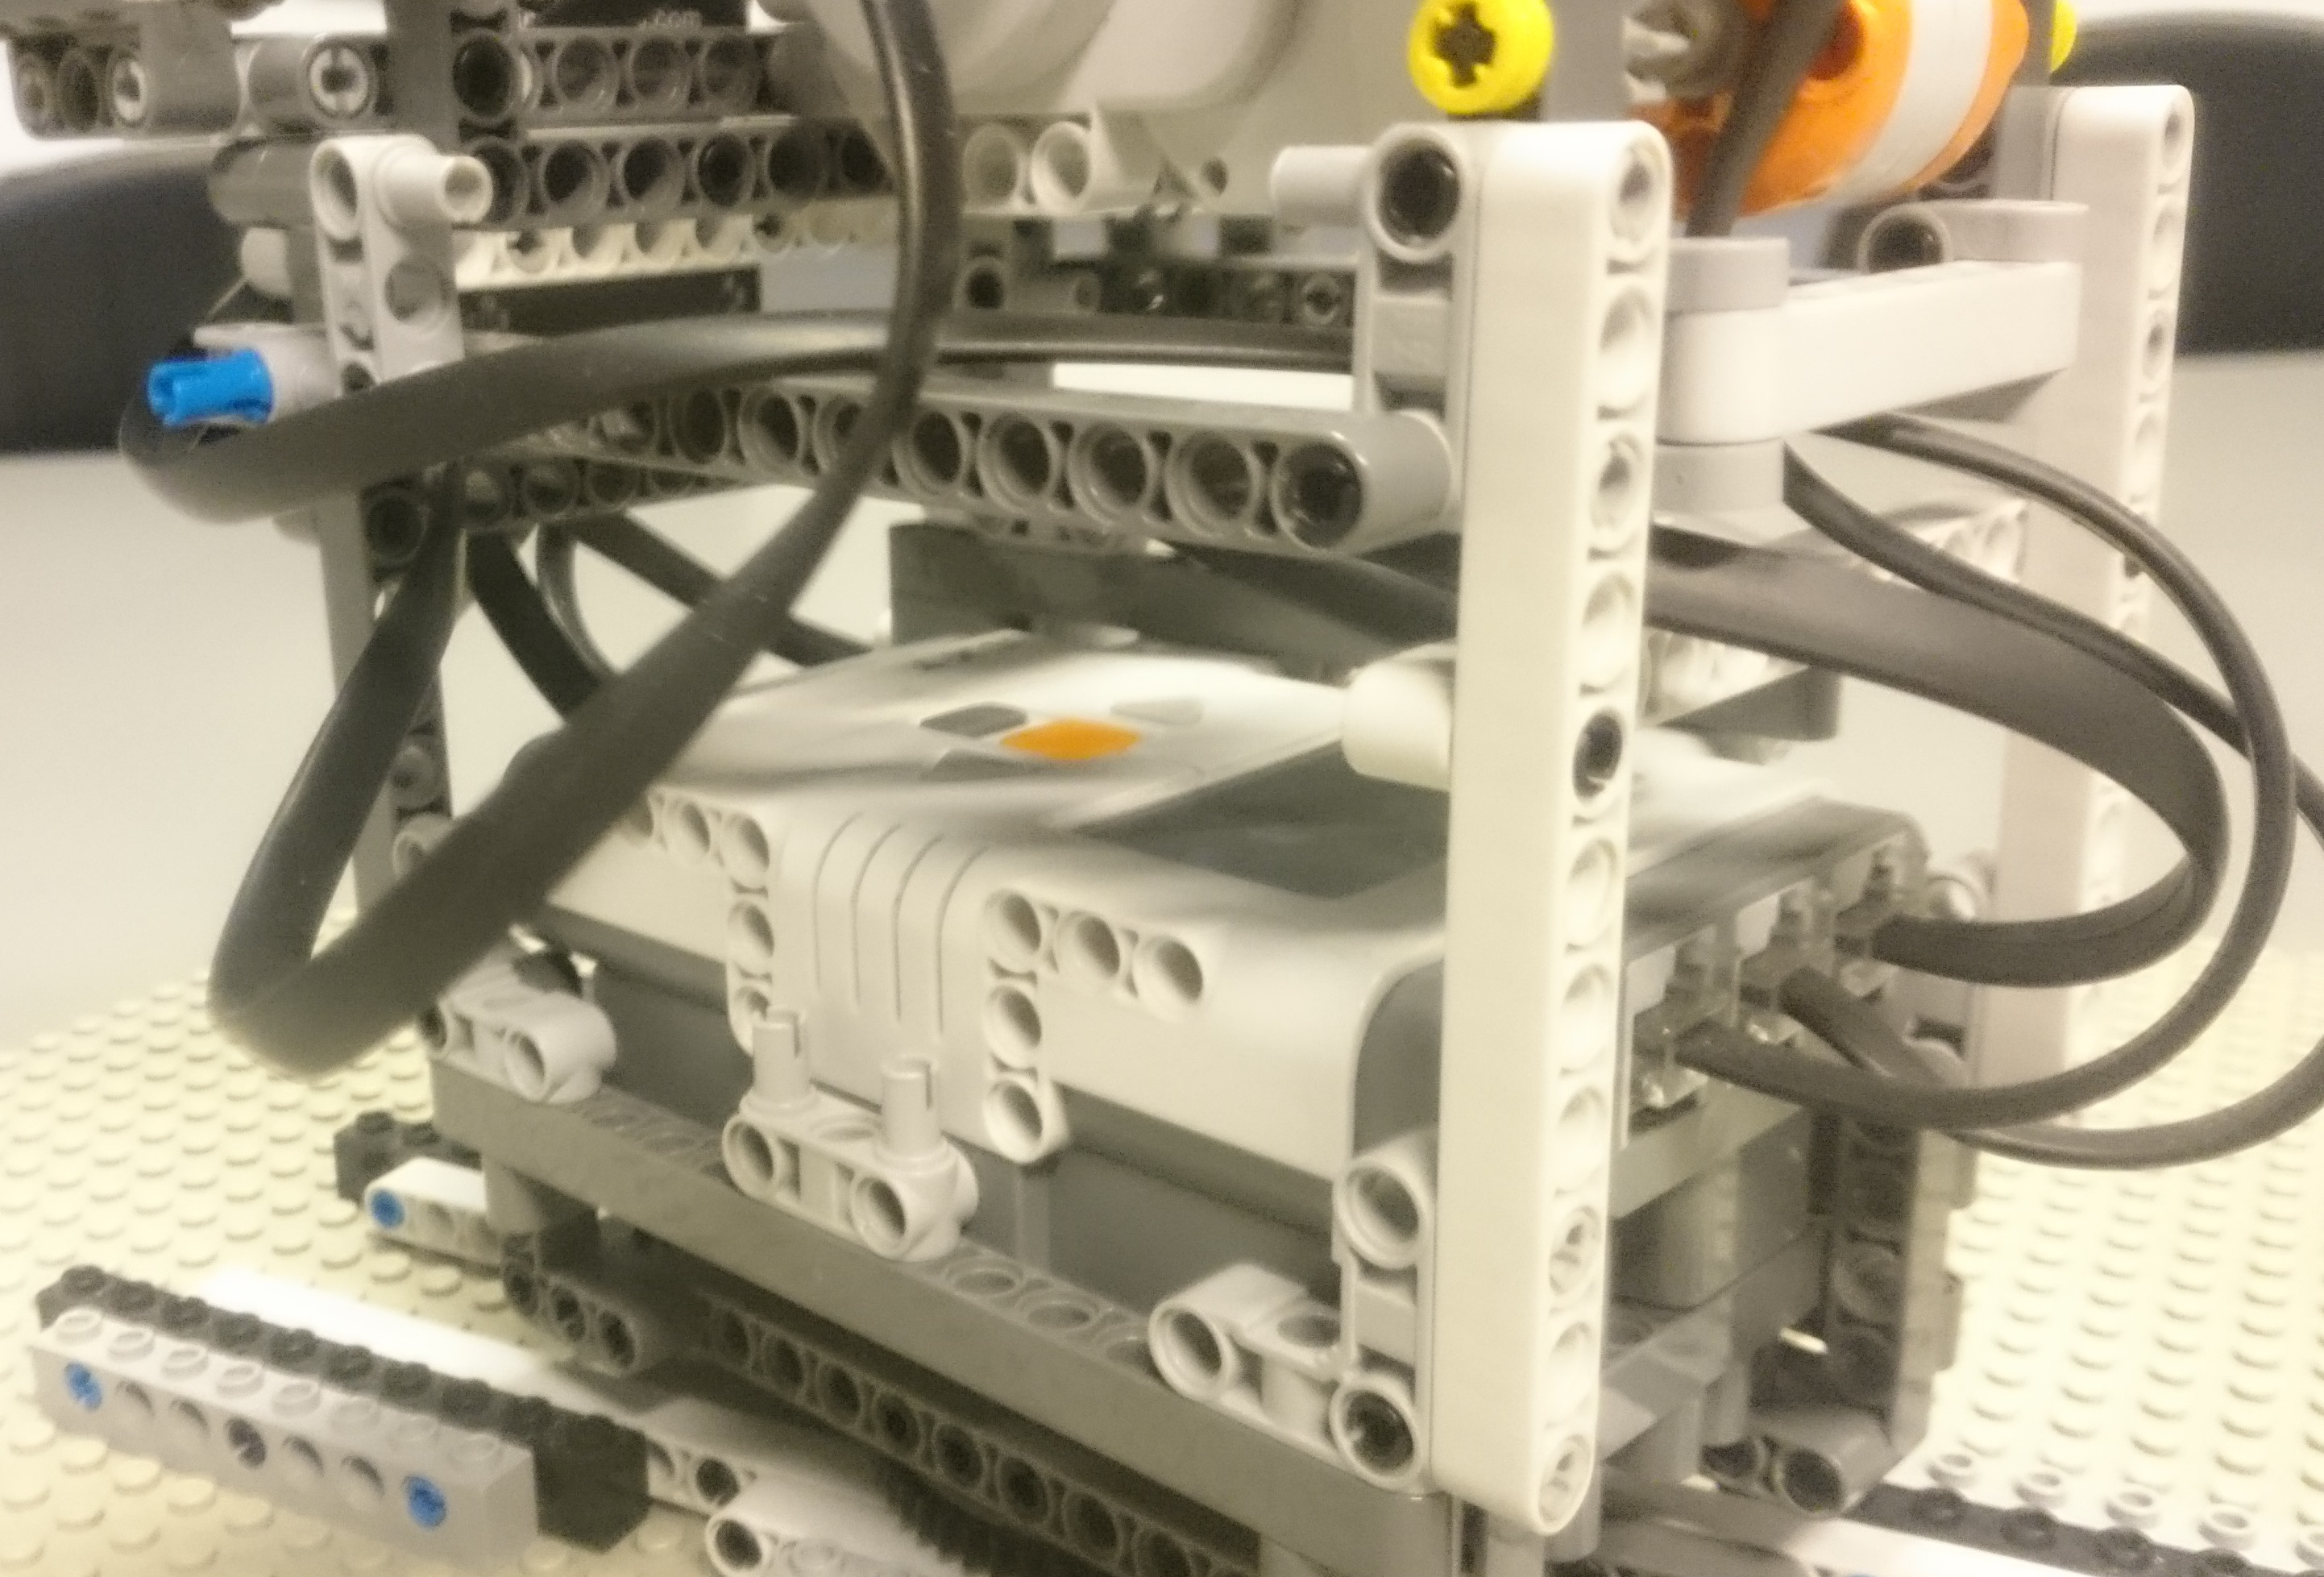
\includegraphics[scale=0.08]{figures/FrameMech.JPG} 

\begin{itemize}
	\item Limited Height
	\item Stable
	\item Inaccesible Buttons
\end{itemize}
\end{frame}

\begin{frame}{Rotational Mechanism}

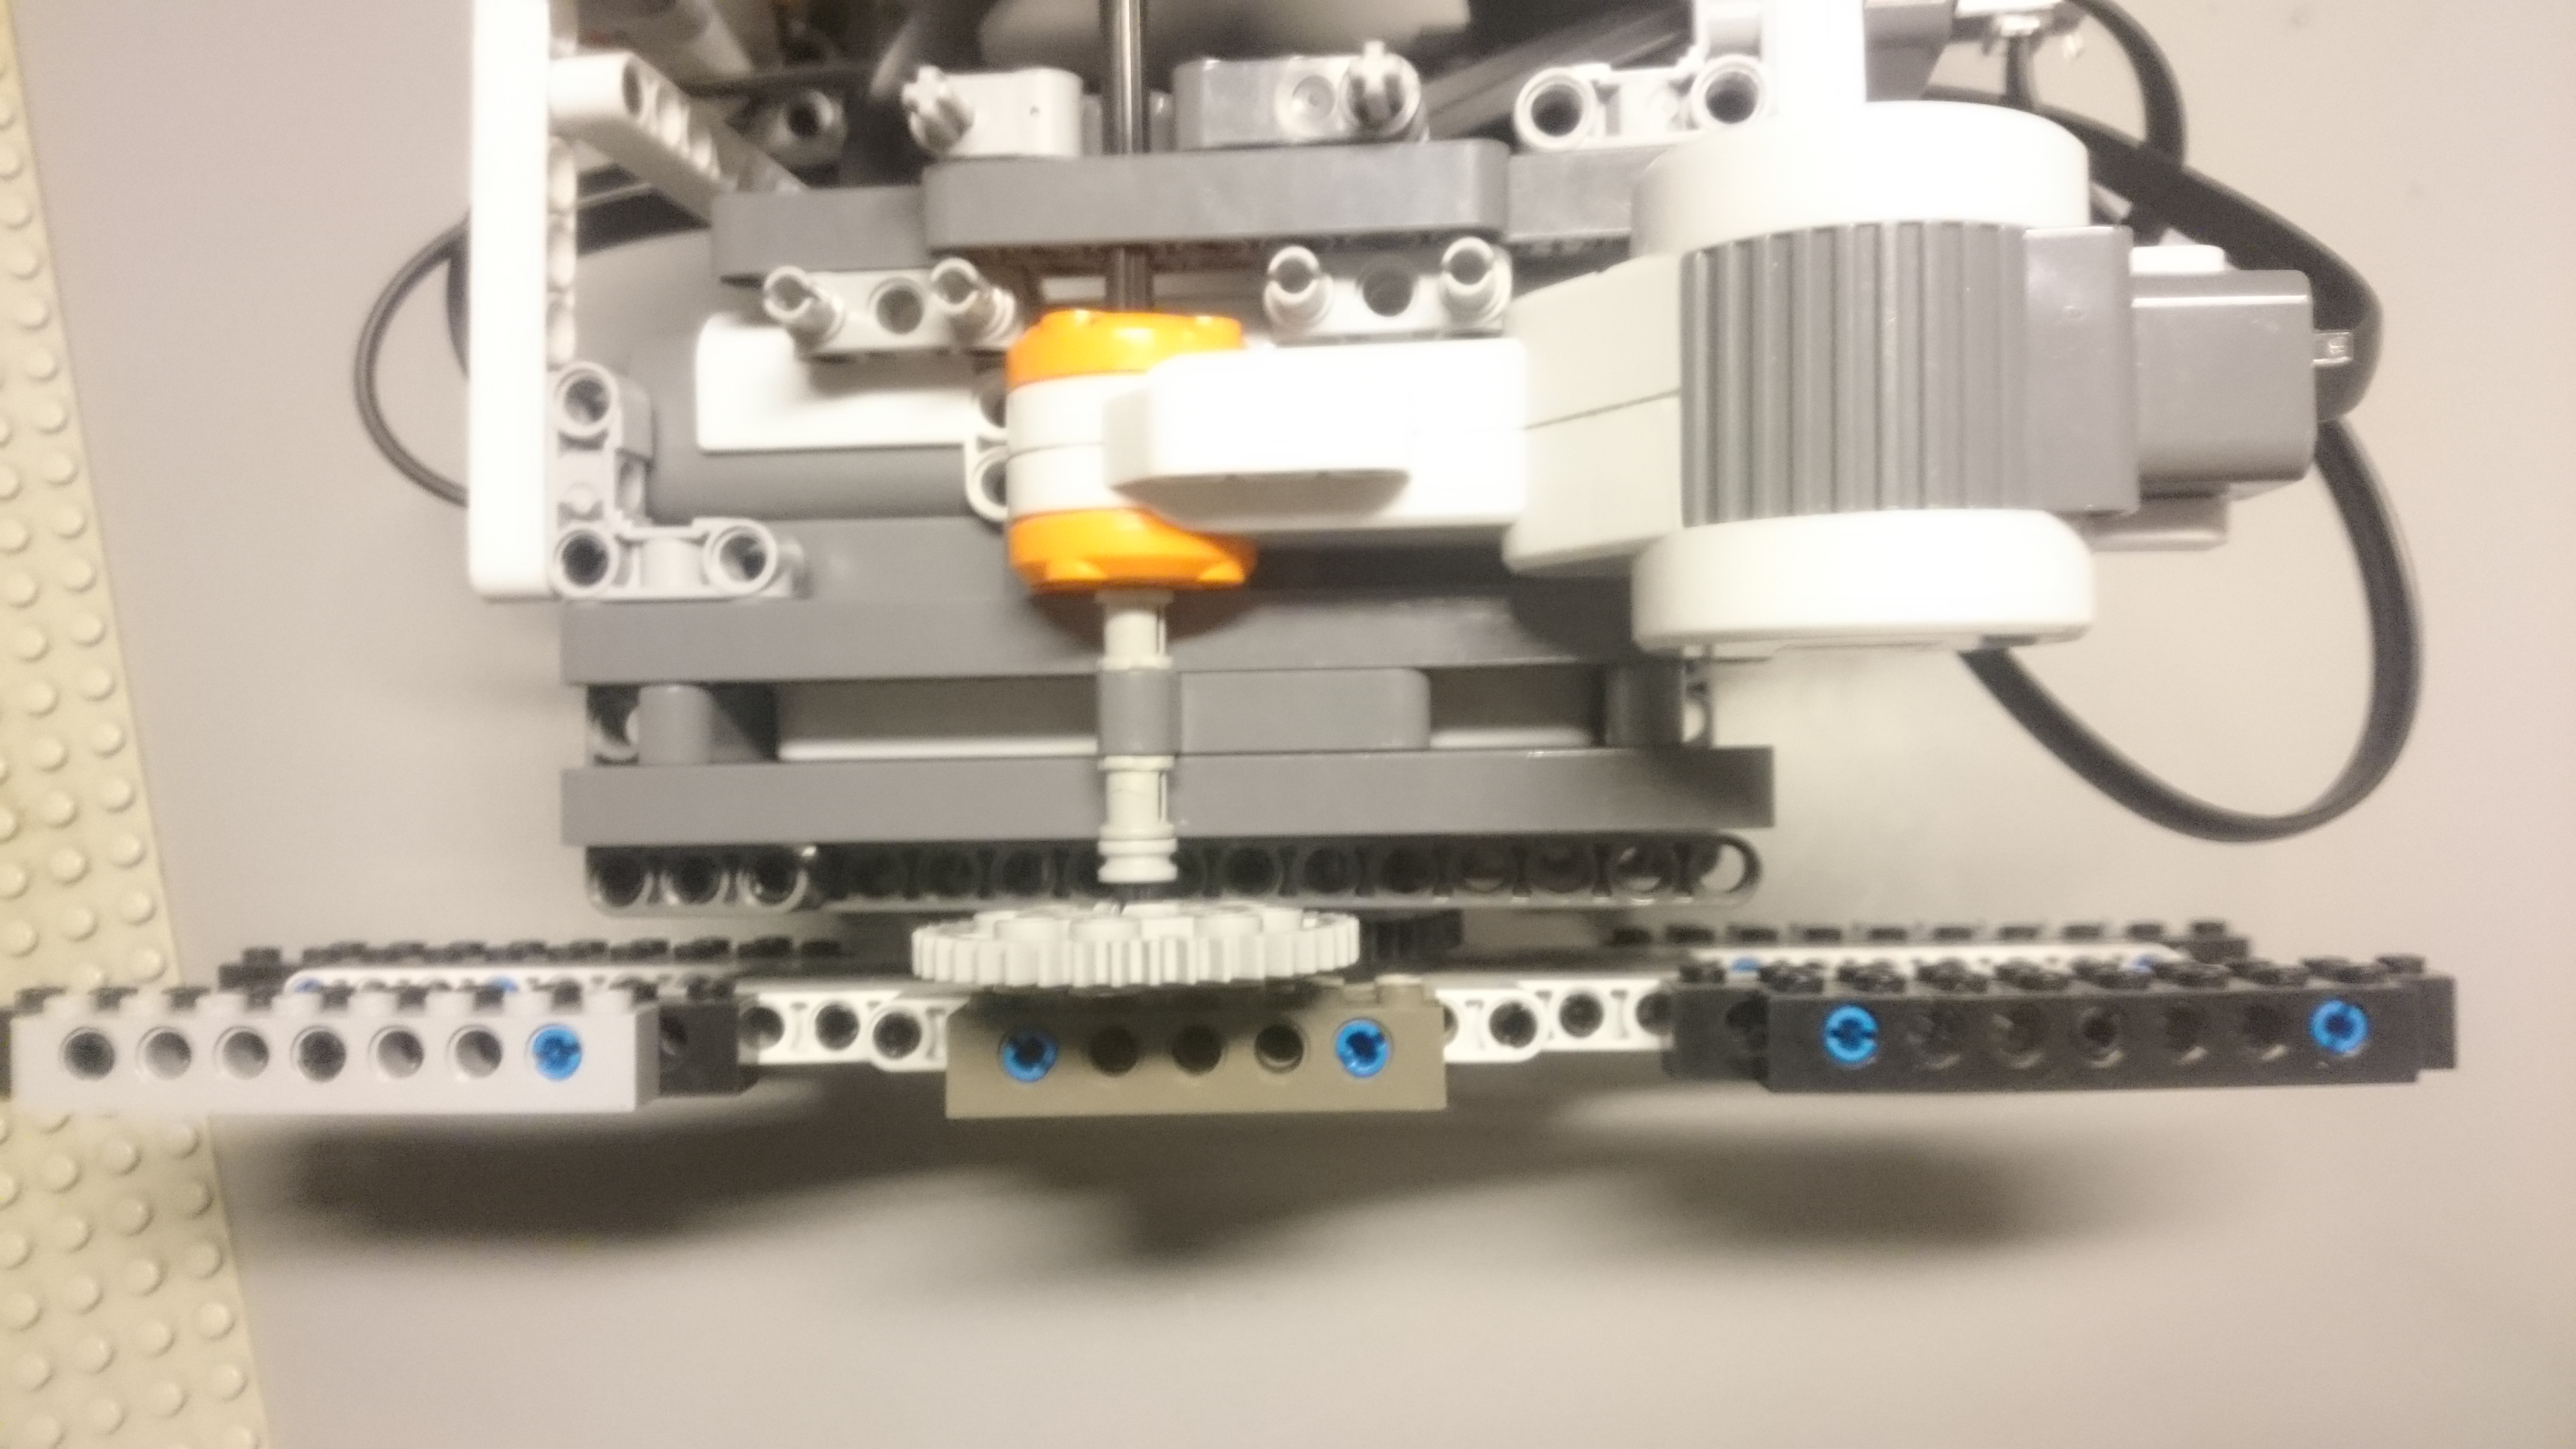
\includegraphics[scale=0.065]{figures/RotMech.JPG} 

\begin{itemize}
    \item Simple Rotational Point 
	\item Somewhat Stable
	\item Limitations
		\begin{enumerate}
  			\item Cables
  			\item Gearing
  			\item Motor Placement
		\end{enumerate}
\end{itemize}
\end{frame}

\begin{frame}{Final Turret}
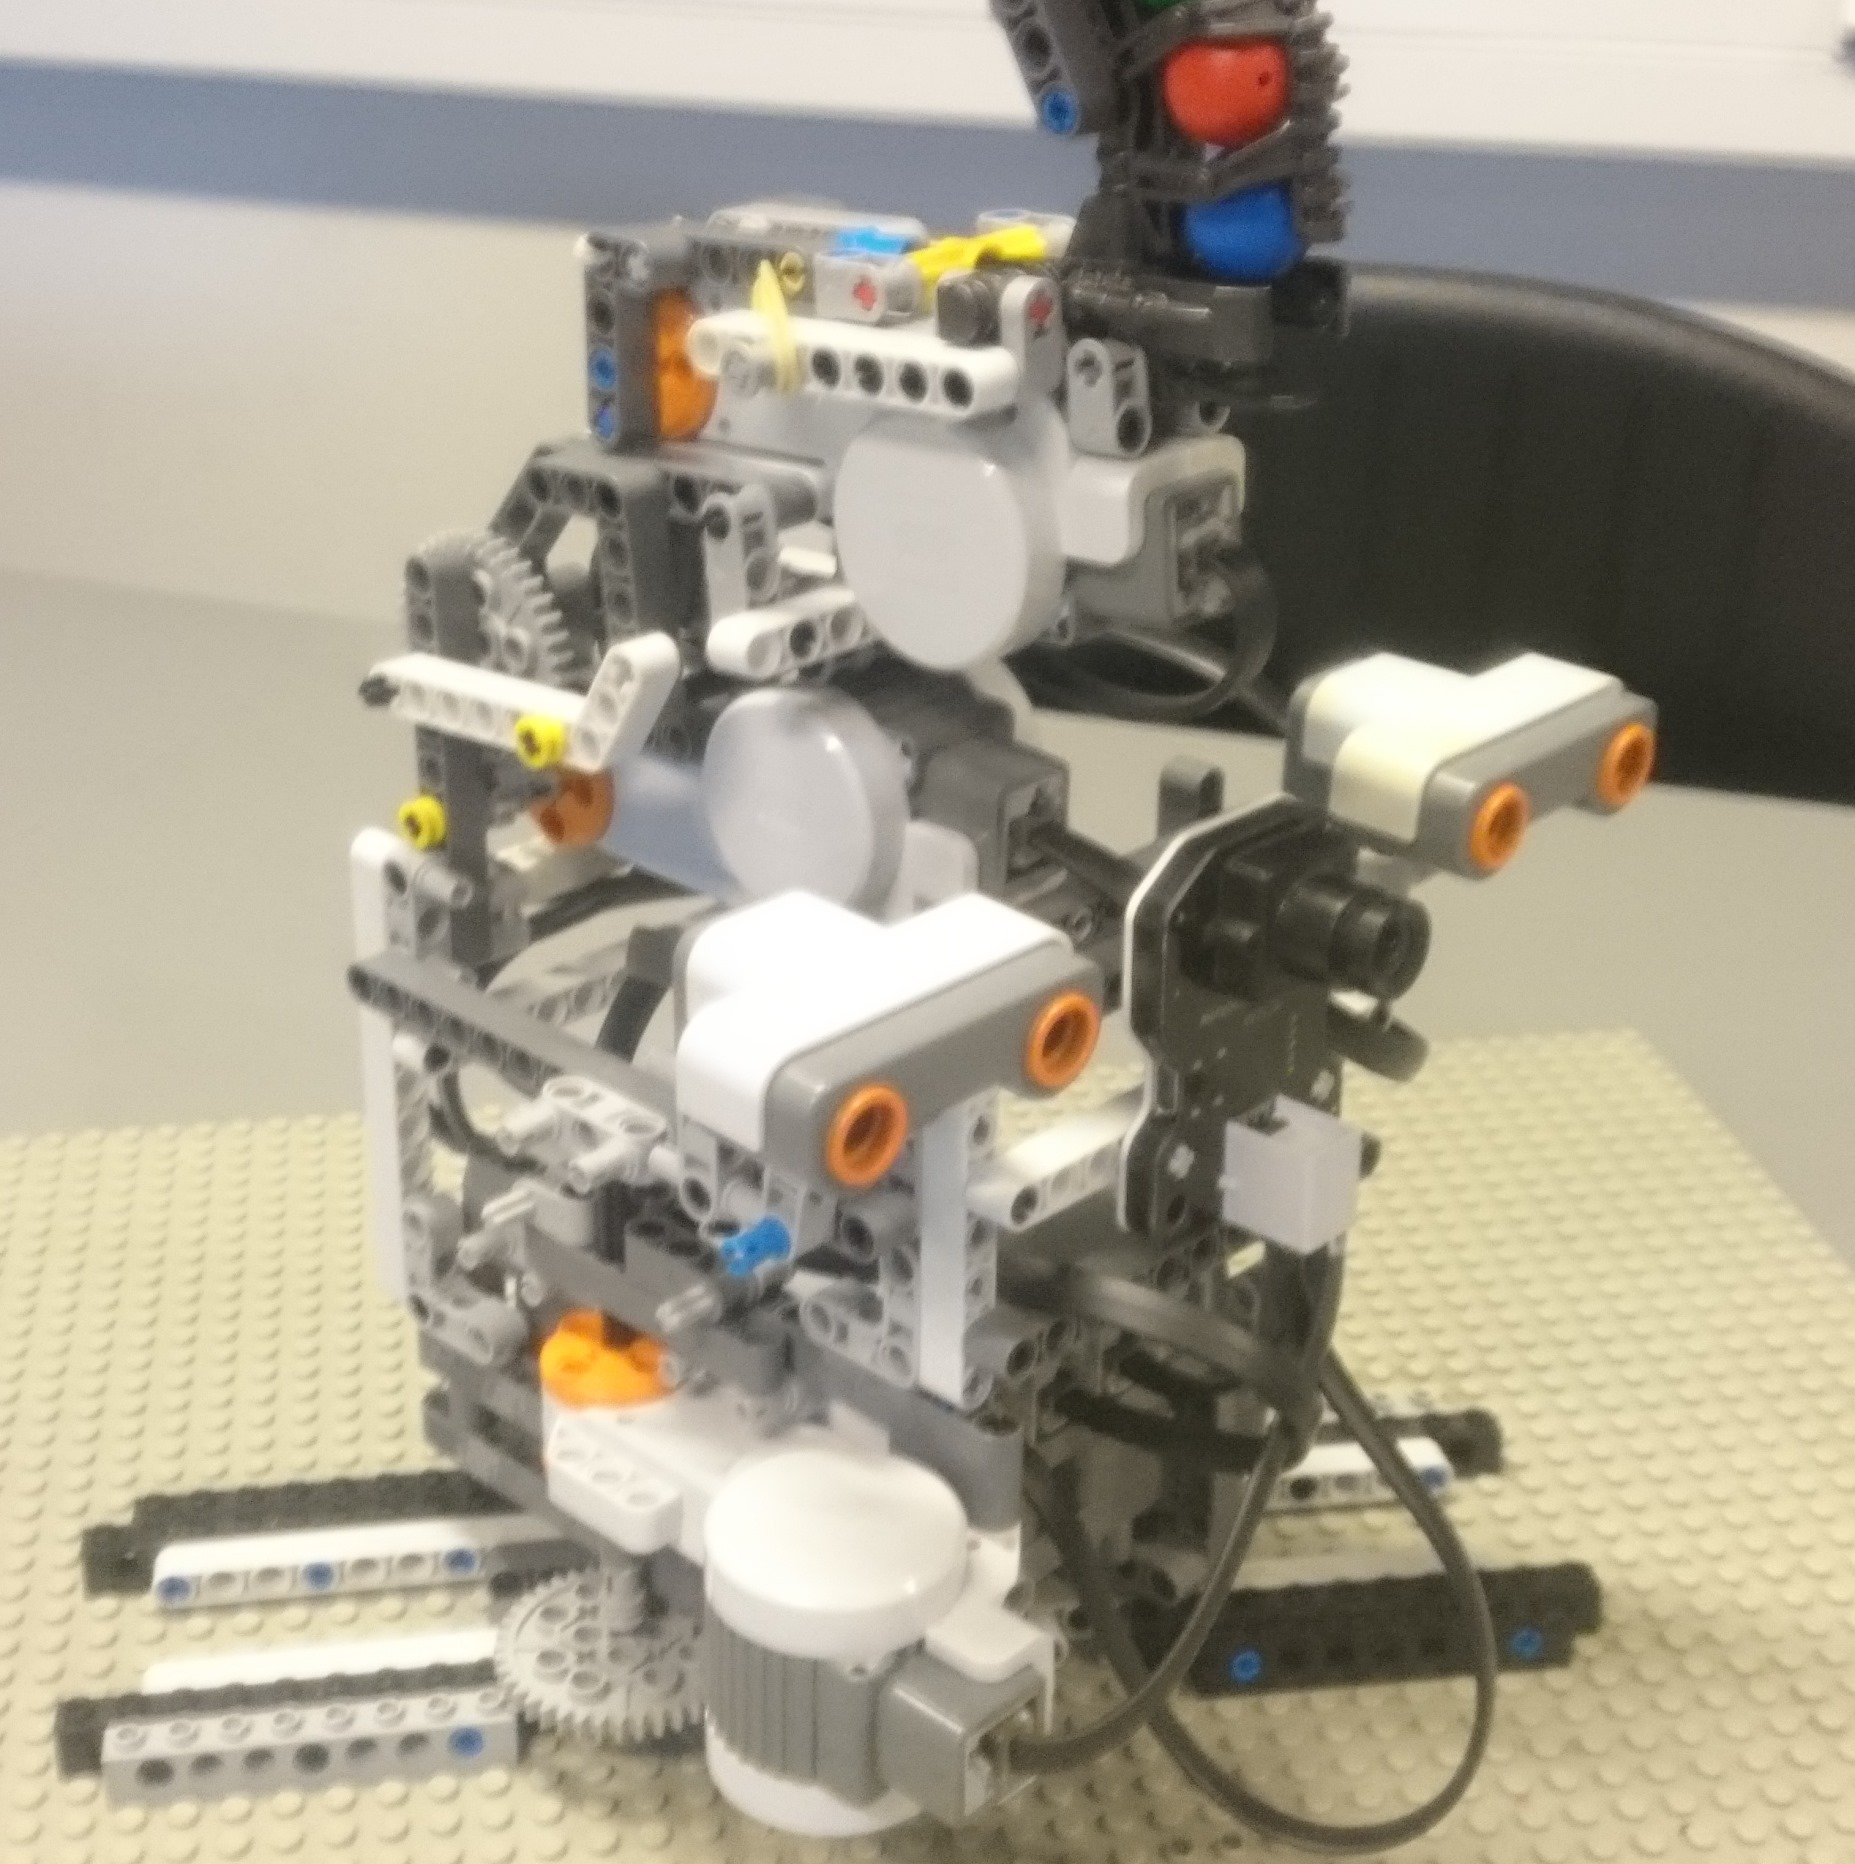
\includegraphics[scale=0.1]{figures/GlorTurret.JPG}  
\end{frame}

%-------------------------------- FRAME 3 --------------------------------
\subsection{Target Design} 
\begin{frame}{Target Requirements}
\begin{itemize}
    \item Predictable Movement
    	\begin{enumerate}
    	    \item Constant Speed 
  			\item Minimal Acceleration
		\end{enumerate}
    \item Move in Straight Line
    	\begin{enumerate}
  			\item No need to turn
  			\item Simple to program
		\end{enumerate}
    \item Recognizable by Camera
    	\begin{enumerate}
  			\item Size
  			\item Colour
  			\item Shape
		\end{enumerate}
\end{itemize}
\end{frame}

\begin{frame}{Final Target Design}

\begin{itemize}
    \item Speed Test
    	\begin{enumerate}
  			\item Unnoticable Acceleration
		\end{enumerate}
    \item Direction
    	\begin{enumerate}
  			\item Somewhat straight line
  			\item Problem with wheels
		\end{enumerate}
	\item Target Body
		\begin{enumerate}
  			\item Large Can
  			\item Bright Red
  			\item Hexagonal Shape
		\end{enumerate}
\end{itemize}
\end{frame}

\begin{frame}{Final Target Design}
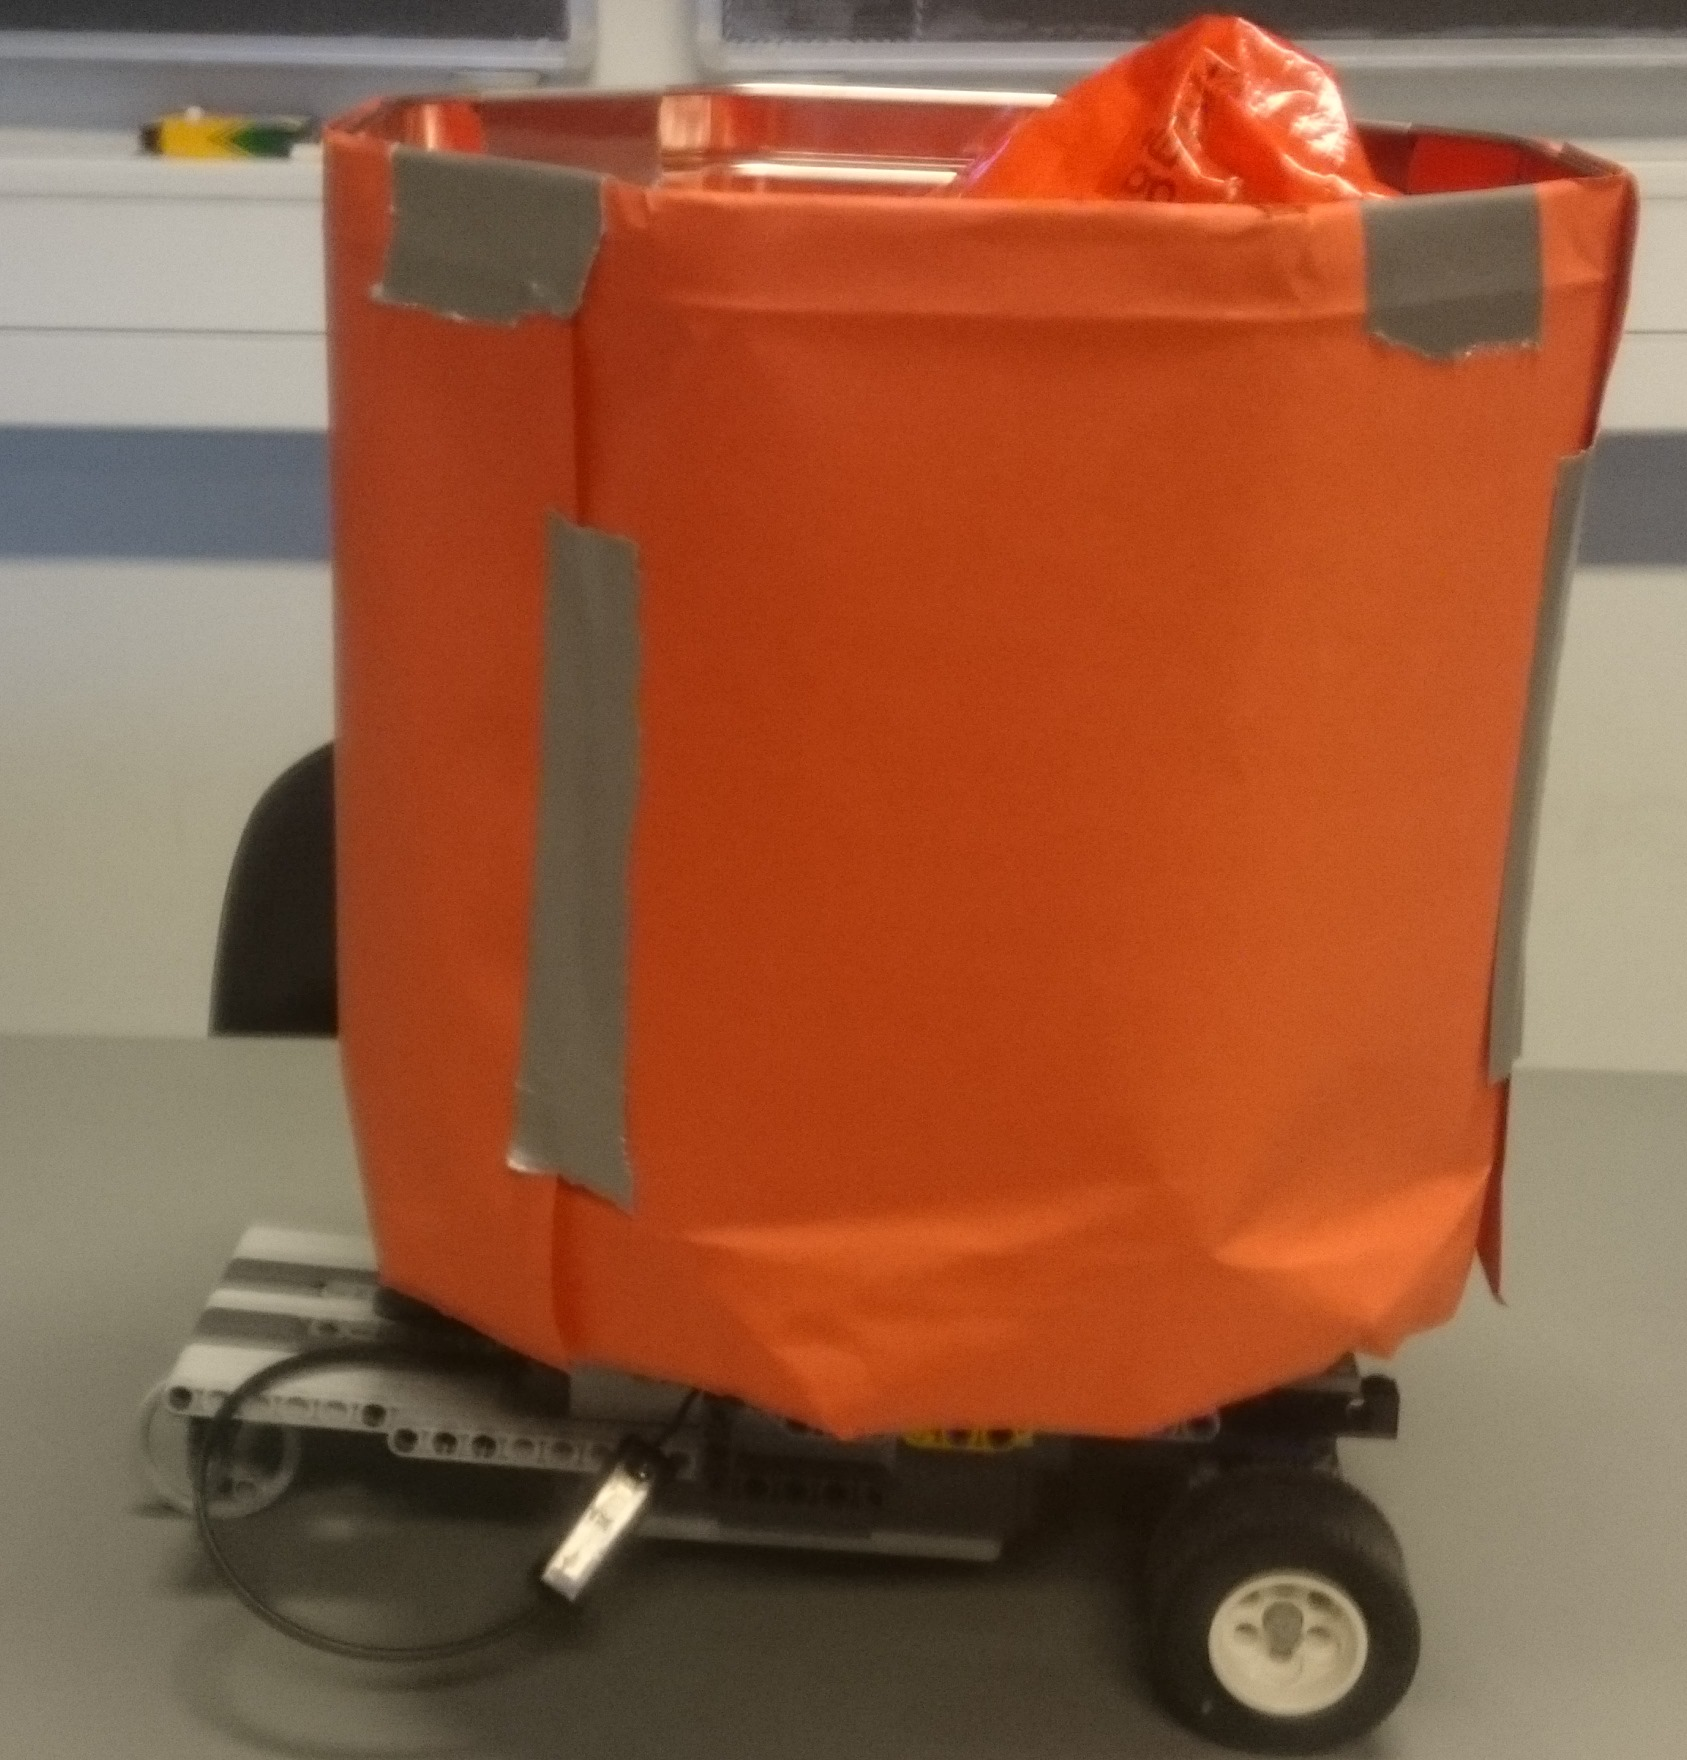
\includegraphics[scale=0.1]{figures/GlorTarget.JPG}
\end{frame}







\section{Jonathan}
\subsection{Overview}
\begin{frame}{Jonathan: Overview}
\begin{itemize}
\item Network Structure
\item Constructing the Tables
\item The Resulting Network
\item Implementation of the Network
\end{itemize}
\end{frame}

% \subsection{Network Structure}
% \begin{frame}{Network Structure}
% \begin{itemize}
% \item What does the network look like?
% \item Which features are used and how are their domains defined?
% \end{itemize}
% \begin{figure}
%   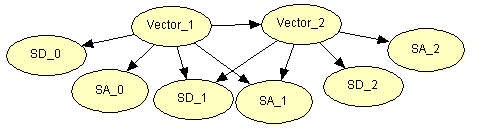
\includegraphics[scale=0.8]{figures/BNDone.PNG}
% \end{figure}
% \end{frame}
\subsection{Network Structure}
\begin{frame}{Network Structure}
\begin{itemize}
\item What does the network look like?
\item Which features are used and how are their domains defined?
\end{itemize}

\begin{figure}
  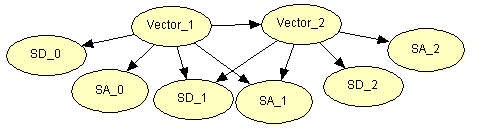
\includegraphics[scale=0.8]{figures/BNDone.PNG}
\end{figure}

\begin{itemize}
  \item Vector - The vector the target is travelling at
  \item SA - The angle at which the target is sensed
  \item SD - The distance to the target
\end{itemize}
\end{frame}

\begin{frame}{Network Structure}
\begin{itemize}
 \item Vector - The vector the target is travelling at
 \item SA - The angle at which the target is sensed
 \item SD - The distance to the target
\end{itemize}

\begin{figure}
  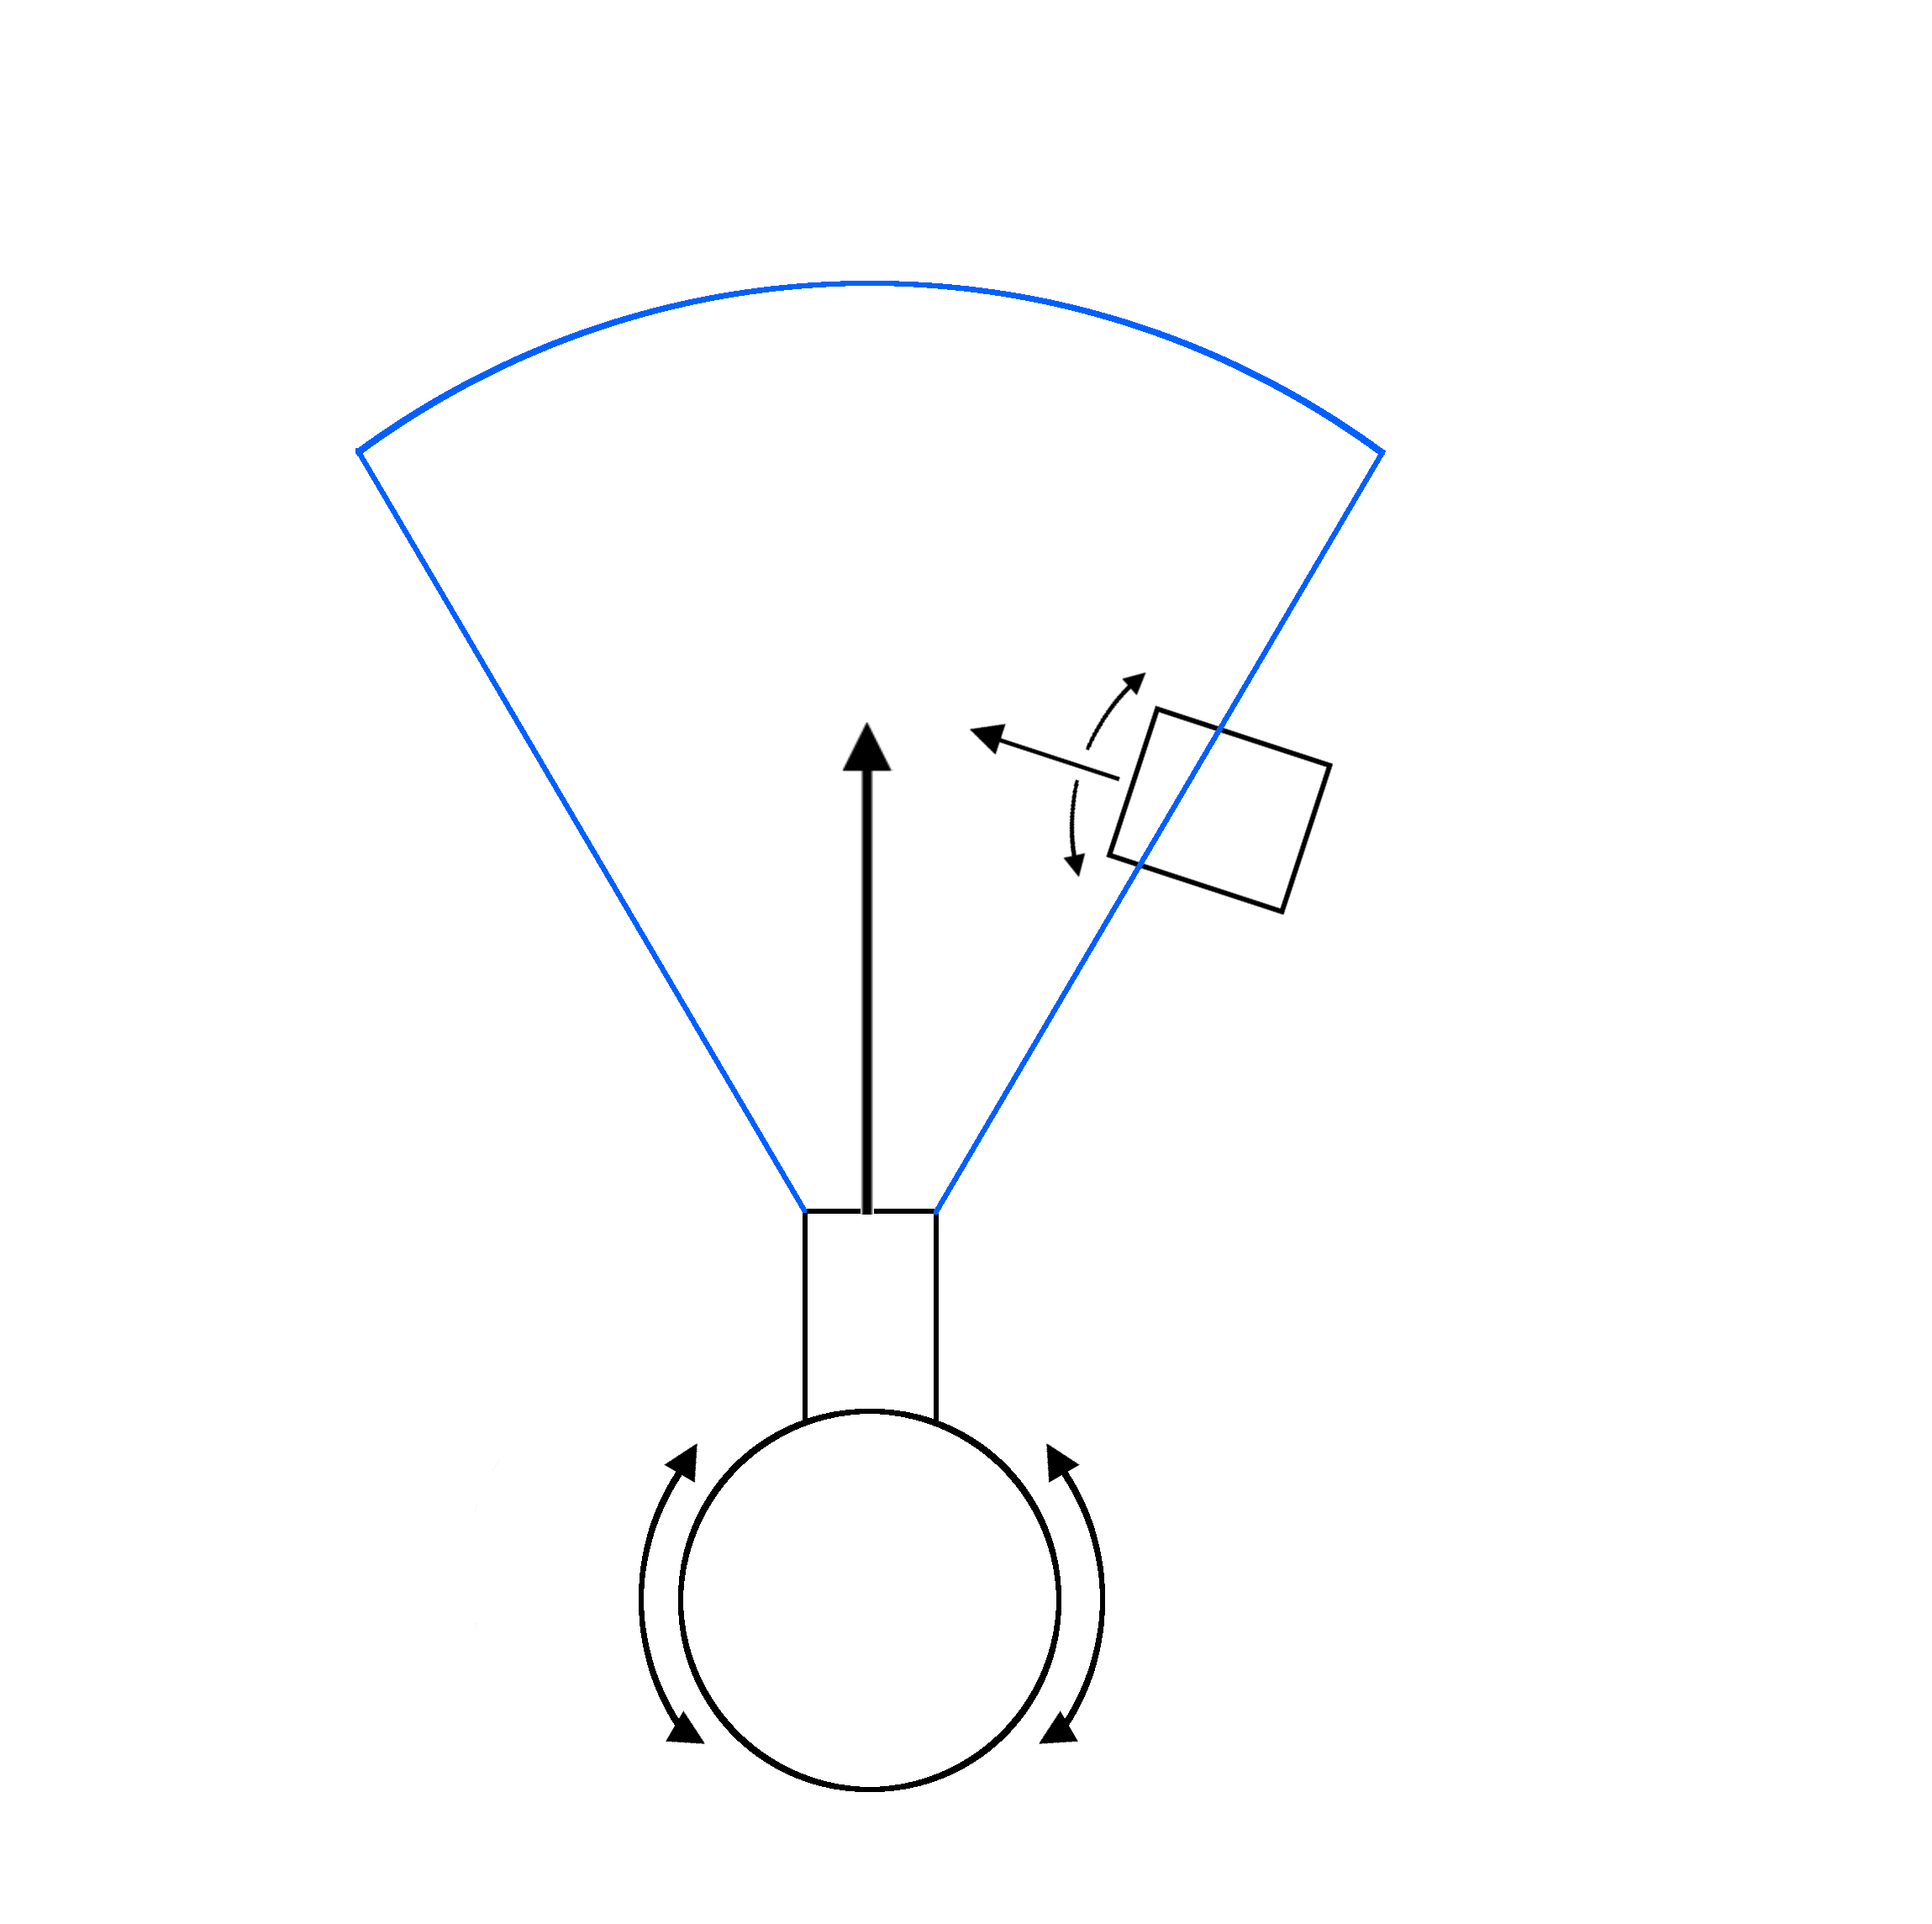
\includegraphics[scale=0.2]{figures/richPic3P5.PNG}
\end{figure}
\end{frame}


\begin{frame}{Network Structure}
\begin{itemize}
 \item Vector - The vector the target is travelling at
 \item SA - The angle at which the target is sensed
 \item SD - The distance to the target
\end{itemize}

\begin{table}
\begin{tabular}{l|l|l}
State & Angle (deg) & Distance (cm) \\ \hline
1     & -30 - 0     & 0 - 60        \\
2     & 0 - 30      & 60 - 75       \\
3     & 30 - 60     & 75 - 90       \\
4     & 60 - 90     & 90 - 105      \\
5     & 90 - 330    & 105 - 255     
\end{tabular}
\end{table}
\end{frame}

\subsection{Constructing the Tables}
\begin{frame}{Constructing the Tables}
\begin{itemize}
\item How was it done? 
\begin{figure}
  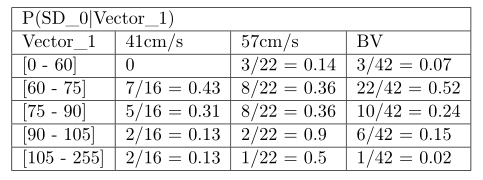
\includegraphics[scale=0.6]{figures/SD0GivenV1.PNG}
\end{figure}

%\item Was the methodology flawed?
\end{itemize}
\end{frame}


\subsection{The Resulting Network}
\begin{frame}{The Resulting Network}
\begin{itemize}
\item Problems with changing vectors
\begin{figure}
  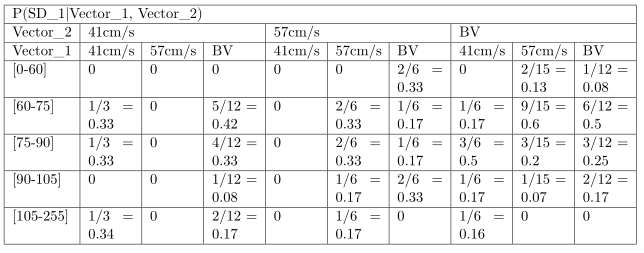
\includegraphics[scale=0.4]{figures/SD1GivenV1V2.PNG}
\end{figure}
\item How can we work around this?
\begin{itemize}
  \item Expanded movement options
  \item Complete rework
  \end{itemize}
\end{itemize}
\end{frame}


\subsection{Implementation of the Belief Network}
\begin{frame}{Implementation of the Belief Network}
\begin{itemize}
\item Have a scaled down version of the network on the NXT
\item Set up a connection to a PC for processing power
\begin{itemize}
   \item Bluetooth vs Serial connection
   \item Defeats the purpose of an embedded system?
   \end{itemize}
\end{itemize}
\end{frame}

\section{Simon}
\subsection{Overview}
\begin{frame}{Simon: Overview}
	\begin{itemize}
	  \item Programming language
	  \item Hardware/software architecture
	  \item Physics implementation
	\end{itemize}
\end{frame}

\subsection{Programming Language}
\begin{frame}{Programming Language}
	\begin{itemize}
	  \item Choosing a programming language
	  \begin{itemize}
	  	\item NXC
	  	\item Pros
	  	\begin{itemize}
	  	  \item Low level 
	  	  \item C-like
	  	\end{itemize}
	  	\item Cons
	  	\begin{itemize}
	  	  \item Bad documentation
	  	  \item No control over the scheduler
	  	  \item No unit test environment
	  	  \item No debugger
	  	\end{itemize}
	  \end{itemize}
	  \item Alternatives
	  \begin{itemize}
	    \item leJos
	    \item ROBOTC
	  \end{itemize}
	\end{itemize}
\end{frame}

\subsection{Hardware/Software Architecture}
\begin{frame}{Hardware/Software Architecture}
\begin{onlyenv}
\only<1>{
\begin{itemize}
  \item Hardware Architecture 
\end{itemize}
	\begin{figure}[H]
  		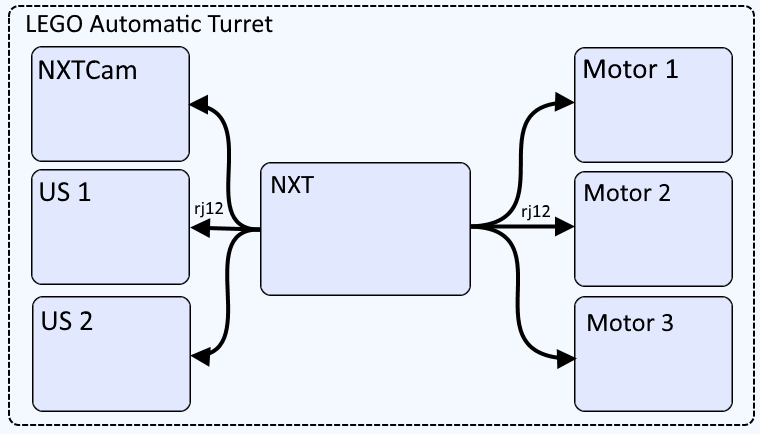
\includegraphics[scale=0.45]{figures/HARCH.png}
	\end{figure}
	}
\only<2>{
\begin{itemize}
  \item Software Architecture
  \item Calls through the software
\end{itemize}
	\begin{figure}[H]
		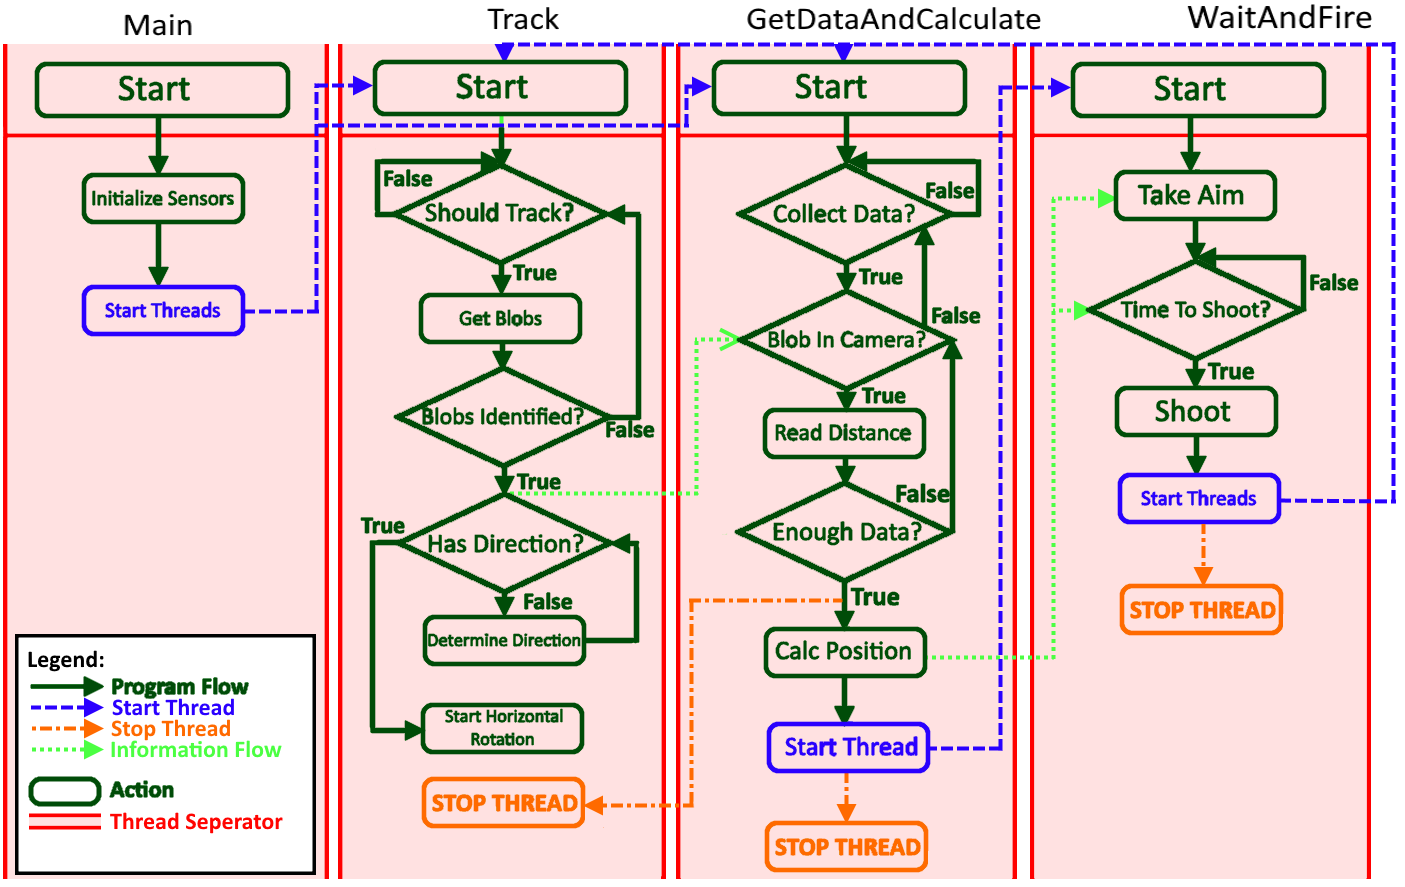
\includegraphics[scale=0.26]{figures/SequenceDiagram.png}
	\end{figure}
}
\end{onlyenv}
\end{frame}

\subsection{Physics Implementation}
\begin{frame}{Physics Implementation}
\begin{equation}\label{locEq3}
a_{positive}=90+(tan^{-1}(\frac{y_{pos}}{x_{pos}}))*(-1)
\end{equation} 
\begin{equation}\label{locEq4}
a_{negative}=(90-(tan^{-1}(\frac{y_{pos}}{x_{pos}})*(-1))*(-1)
\end{equation} 

\begin{figure}[H]
	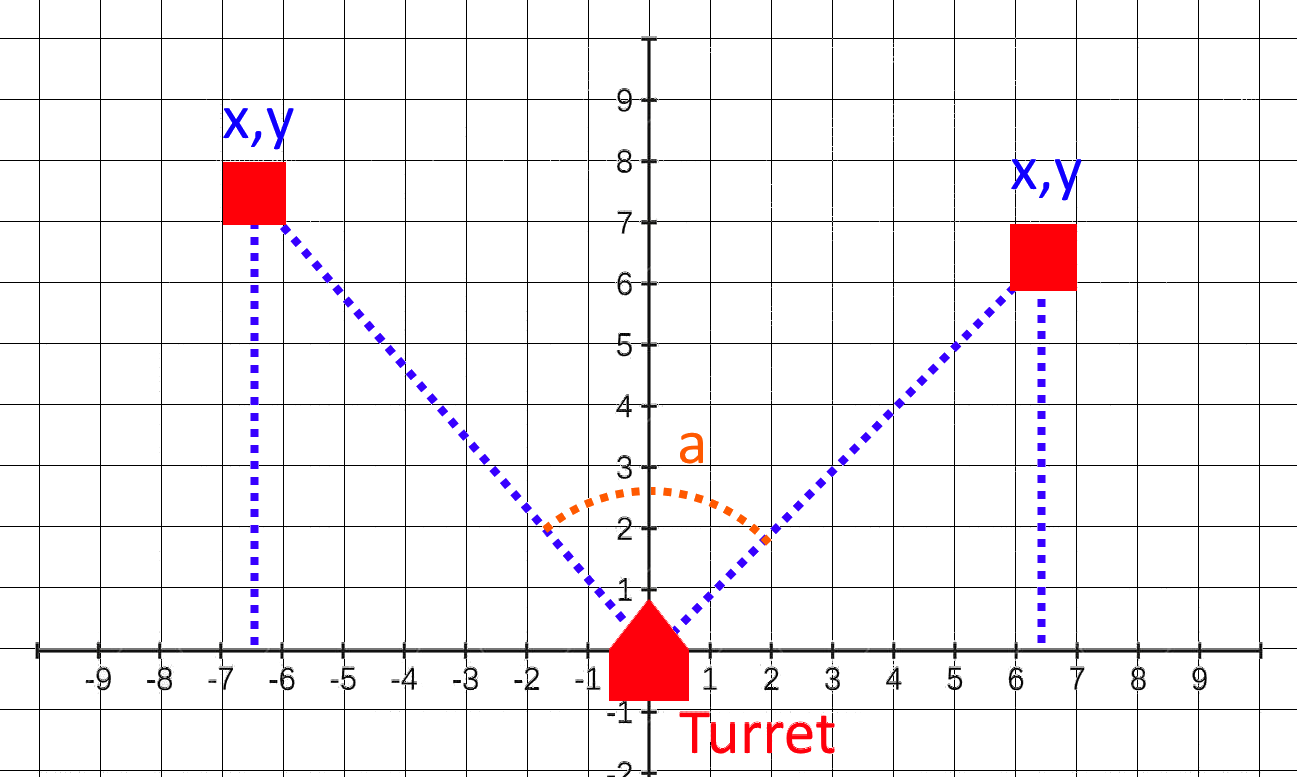
\includegraphics[scale=0.25]{figures/CoordinateSystem3.png}
\end{figure}

\end{frame}

\begin{frame}[fragile]{Physics Implementation}
\begin{center}
\begin{minipage}[H]{0.9\linewidth}
 \begin{lstlisting}
PosData CalcFuturePos(DirectionVector vector, unsigned long time){
   PosData futurePosition;
   float tanInput = 0;
   futurePosition.xPos = vector.xPos + vector.speedX * time;
   futurePosition.yPos = vector.yPos + vector.speedY * time;
   futurePosition.time = CurrentTick() + time;

   tanInput = futurePosition.yPos / futurePosition.xPos;
   if(futurePosition.xPos >= 0)
        futurePosition.angle = 90+(atand(tanInput))*(-1);
   else
        futurePosition.angle = (90-(atand(tanInput))*(-1))*(-1);
   
   return futurePosition;
}
 \end{lstlisting} 
\end{minipage}
\end{center}
\end{frame}
\section{Christoffer}
% \begin{frame}{Christoffer}
% \begin{itemize}
%   \only<1->{\item This}
%   \only<2->{\item is}
%   \only<3->{\item a}
%   \only<4>{\item test}
% \end{itemize}
% \end{frame}

\begin{frame}{Christoffer}
\begin{itemize}
  \item The tasks of our program
  		\begin{enumerate}
  			\item What is each tasks purpose
  			\item Key implementation points of each task
  			\item Why they are implemented as they are  
		\end{enumerate}
  \item Unit tests
  		\begin{enumerate}
  			\item How have we unit tested
  			\item The framework
  			\item The results of the test
		\end{enumerate}
  \item The final test of the turret
%   		\begin{enumerate}
%   			\item 
% 		\end{enumerate}
\end{itemize}
\end{frame}

\subsection{Tasks}
\begin{frame}{Tasks}
\begin{itemize}
  \item Main
  \item Track
  \item GetDataAndCalculate
  \item WaitAndFire
\end{itemize}
\end{frame}

\begin{frame}[fragile]{Main}
\only<1-3>{
\begin{itemize}
  \item Purpose
  	\only<2>{
  	\begin{itemize}
  		\item Start tasks
  		\item Setup
  	\end{itemize}
  	}
  \only<3>{\item Key implementation points}
\end{itemize}
}
\begin{onlyenv}<4>
\begin{center}
\begin{minipage}[H]{0.9\linewidth}
\begin{lstlisting}
PosRegEnable(ROTATE_MOTOR);
PosRegEnable(ANGLE_MOTOR);
SetMotorRegulationTime(10);
NXTCam_Init(CAM_PORT, CAM_ADDR);
NXTCam_SendCommand(CAM_PORT, CAM_ADDR, 'A'); 
NXTCam_SendCommand(CAM_PORT, CAM_ADDR, 'E');
SetSensorUltrasonic(SENSOR_LEFT);
SetSensorUltrasonic(SENSOR_RIGHT);
Precedes(Track,GetDataAndCalculate);
\end{lstlisting} 
\end{minipage}
\end{center}
\end{onlyenv}
\end{frame}

\begin{frame}[fragile]{Track}
\only<1-3>{
\begin{itemize}
  \item Purpose
  	\only<2>{
  	\begin{itemize}
  		\item Track targets
  		\item Information sharing
  	\end{itemize}
  	}
  \only<3>{\item Key implementation points}
\end{itemize}
}
\begin{onlyenv}<4>
\begin{center}
\begin{minipage}[H]{0.9\linewidth}
\begin{lstlisting}
while(track){
	NXTCam_GetBlobs(CAM_PORT, CAM_ADDR, nblobs, bc, bl, bt, br, bb);
    if(nblobs > 0){
    	blobInCam = true;
        ....
        if(lib_direction != NO_DIRECTION){
        	tempSpeed = GetSpeed(blobCenter );
            if(tempSpeed > 0 && lib_direction == RIGHT_DIRECTION)
            	OnFwd(ROTATE_MOTOR, tempSpeed);
            else if(tempSpeed < 0 && lib_direction == LEFT_DIRECTION)
            	OnFwd(ROTATE_MOTOR, tempSpeed);
        }
	}else{
    	blobInCam = false;
        ...
    	Off(ROTATE_MOTOR);
	}
    DetermineDirection(blobCenter, oldBlobCenter, directionCount);
}
\end{lstlisting} 
\end{minipage}
\end{center}
\end{onlyenv}
\end{frame}

\begin{frame}[fragile]{GetDataAndCalculate}
\only<1-3>{
\begin{itemize}
  \item Purpose
  	\only<2>{
  	\begin{itemize}
  		\item Collect data
  		\item Calculate vectors and positions
  		\item Determine the shooting position
  	\end{itemize}
  	}
  \only<3>{\item Key implementation points}
\end{itemize}
}
\begin{onlyenv}<4>
\begin{center}
\begin{minipage}[H]{0.9\linewidth}
\begin{lstlisting}
while(collecting){
	if(blobInCam){
        if(length != NO_DATA){
            if(MakePosData(length,GetMotorAngle(),CurrentTick(),tempPosData)){
            	posData[posDataCounter] = tempPosData;
                posDataCounter++;
            }
            if(posDataCounter == DATASETS_NEEDED_TO_CALCULATE){
				track = false;
                Off(ROTATE_MOTOR); 
                StopTask(Track);
                DirectionVector vector = CalcDirVector(posData,posDataCounter);
                fire = CalcFireData(CalcFuturePos(vector,MILLISECONDS_TO_HIT));
                StartTask(WaitAndFire);
            }
    	}
	}
}
\end{lstlisting} 
\end{minipage}
\end{center}
\end{onlyenv}
\end{frame}

\begin{frame}[fragile]{WaitAndFire}
\only<1-3>{
\begin{itemize}
  \item Purpose
  	\only<2>{
  	\begin{itemize}
  		\item Wait until the calculated time
  		\item Shoot the target at the calculated position
  		\item Reset the turret
  	\end{itemize}
  	}
  \only<3>{\item Key implementation points}
\end{itemize}
}
\begin{onlyenv}<4>
\begin{center}
\begin{minipage}[H]{0.9\linewidth}
\begin{lstlisting}
collecting = false;
LoadRound();
Off(ROTATE_MOTOR);
RotateH(fire.angleH);
Angle(fire.angleV);
while(true){
	if(CurrentTick() >= fire.timeToHit && !alreadyFired){
    	alreadyFired = true;
        Fire();
        break;
    }
}
Angle(START_ANGLE);
...
Wait(4000);
StartTask(Track);
StartTask(GetDataAndCalculate);
\end{lstlisting} 
\end{minipage}
\end{center}
\end{onlyenv}
\end{frame}

\subsection{Unit Test}
\begin{frame}[fragile]{Unit Test}
\begin{itemize}
  \only<1-2,6-8>{\item How have we tested}
  \only<2-2,6-8>{\item No framework}
  \only<6-8>{\item What have we tested}
  			\only<7>{
  			\begin{enumerate}
  				\item CalcDirVector
  				\item UpperBound
  				\item CheckLength
  				\item GetSpeed
  				\item And more\ldots
  			\end{enumerate}
  			}
  \only<8-9>{\item Results} 
\end{itemize}
\begin{onlyenv}<3>
\begin{center}
\begin{minipage}[H]{0.9\linewidth}
\begin{lstlisting}
bool CombineVectorsTest2(){
	DirectionVector input1;
	input1.speedX = 10;
  	input1.speedY = 10;
  	input1.xPos = 15;
  	input1.yPos = 15;

  	DirectionVector dirVecArray[1];
  	dirVecArray[0] = input1;
  	DirectionVector out = CombineVectors(dirVecArray, 1);

  	if(out.speedX == 10 && out.speedY == 10 && out.xPos == 15, out.yPos == 15){
    	return true;
  	}
  	else {
    	return false;
  	}
}

bool UpperBoundTest(int input, int expected){
	int out = UpperBound(input);

  	return Assert(out, expected);
}
\end{lstlisting} 
\end{minipage}
\end{center}
\end{onlyenv}
\begin{onlyenv}<4>
\begin{center}
\begin{minipage}[H]{0.9\linewidth}
\begin{lstlisting}
task main(){
	unsigned int rtn_code = CreateFile(NAME, SIZE, handle);
   	if (rtn_code == LDR_FILEEXISTS)
     	rtn_code = OpenFileAppend(NAME, SIZE, handle);
  	...
 	if(UpperBoundTest(130, 130)){
    	WriteLn(handle, "UpperBoundTest: Passed");
  	}
 	else{
    	WriteLn(handle, "UpperBoundTest: Failed");
  	}
  	if(UpperBoundTest(240, 144)){
    	WriteLn(handle, "UpperBoundTest2: Passed");
  	}
  	else{
    	WriteLn(handle, "UpperBoundTest2: Failed");
  	}
  	if(CombineVectorsTest2()){
    	WriteLn(handle, "CombineVectorsTest2: Passed");
  	}
  	else{
    	WriteLn(handle, "CombineVectorsTest2: Failed");
  	}
  	...
  	CloseFile(handle);
}
\end{lstlisting} 
\end{minipage}
\end{center}
\end{onlyenv}

\begin{onlyenv}<5>
\begin{itemize}
  \item How have we tested
  \item No framework
  \begin{itemize}
  \item Non testable function
\end{itemize}
\end{itemize}
\begin{center}
\begin{minipage}[H]{0.9\linewidth}
\begin{lstlisting}
float GetMotorAngle(){
    return MotorRotationCount(ROTATE_MOTOR)*0.73;
}
\end{lstlisting} 
\end{minipage}
\end{center}
\end{onlyenv}
\only<9>{
\begin{figure}[H]
  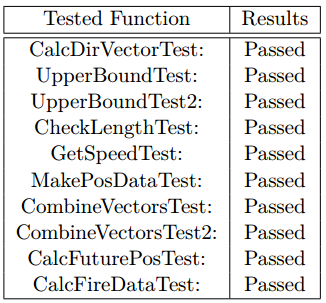
\includegraphics[scale=0.5]{figures/result.png}
\end{figure}
}
\end{frame}

\subsection{Final Test}
\begin{frame}{Final Test}
\begin{itemize}
  \only<1-4>{\item Setup}
  \only<2-4>{\item Execution}
  \only<3-4>{\item Observations}
  \only<4->{\item Result}
  \only<5>{
\begin{figure}[H]
  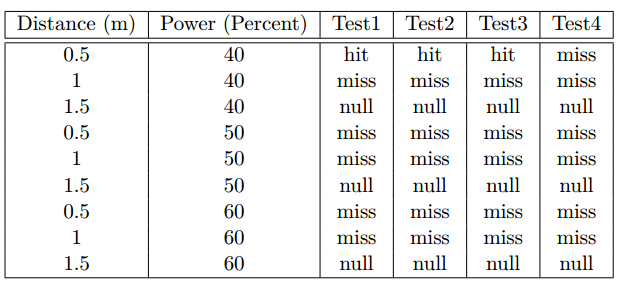
\includegraphics[scale=0.5]{figures/finalTestResult.png}
\end{figure}
}
\end{itemize}
\end{frame}
\section{Michael}
\begin{frame}{Michael}
	\begin{itemize}
		\item Product Demonstration
		\item General Discussion
		\item Final Conclusion
	\end{itemize}
\end{frame}


\subsection{Product Demonstration}


\subsection{Evaluation - General Discussion}
\begin{frame}{Evaluation - Discussion}
	\begin{itemize}
		\item Quantity of Data
		\item Sensor Quality
		\item Machine Intelligence Implementation
		\item Code refactoring
	\end{itemize}
\end{frame}



\subsection{Evaluation - Final Conclusion}
\begin{frame}{Evaluation - Final Conclusion}
	\only<1->{\textit{
		How can an autonomous turret be constructed, designed and imple- mented using the NXT, a camera and a pair of ultrasonic distance sensors. Furthermore, how can a belief network be constructed and used for predicting the position of the target.}
	}
	\only<2->{
		Many of the technical aspects were completed
		\begin{itemize}
			\item Rotating 360 degrees
			\item Capable of firing multiple shots
			\item Verticle angle capable of adjusting shooting length
			\item Capable of working with a target travelling in different directions
		\end{itemize}
	}
	\only<3->{
		But on the other hand
		\begin{itemize}
			\item Only 1 range and speed combination where we actually hit
			\item Currently operating on restricted parameters
		\end{itemize}
	}
\end{frame}
{\aauwavesbg
\begin{frame}[plain,noframenumbering]
  \finalpage{Thank you!}
\end{frame}}
%%%%%%%%%%%%%%%%

\end{document}
